\section{Method}
\label{sec:method}

\subsection{Setup and notation}
\label{sec:setup}

We consider a two-layer GCN for node classification. Let $\Ahat$ be the fixed message-passing
operator, $X$ the node features, and
\begin{equation}
\begin{gathered}
\Bone = \Ahat X W_{1} + b_{1},\qquad H_{1} = \mathrm{relu}(\Bone),\\
\Btwo = \Ahat H_{1} W_{2} + b_{2},\qquad \hat{y} = \arg\max \Btwo .
\end{gathered}
\label{eq:gcn}
\end{equation}
Write $a_{n} \coloneqq \Ahat[n,:]$ for the row of node $n$, $\rhon \coloneqq \lVert a_{n}\rVert_{1}$
its row sum---not $1$, for symmetric normalisation---and $\anorm$ its Euclidean norm. The
derivation only requires $\Ahat$ to be fixed and non-negative; the three operators we test are
symmetric normalisation ($\rho$ mean $0.93$, max $5.75$ on Cora), mean aggregation ($\rho = 1$) and
sum aggregation ($\rho$ up to $169$).

The spiking network keeps the trained weights. Layer~1 is an integrate-and-fire (IF) population with
threshold $\theta$, reset by subtraction, driven by the constant per-step current
$\Bone[n,h] + \beta$:
\begin{equation}
u_{1} \leftarrow u_{1} + \Bone + \beta,\quad
s_{1} = \mathbb{1}\!\left[u_{1} \ge \theta\right],\quad
u_{1} \leftarrow u_{1} - \theta s_{1}.
\label{eq:if}
\end{equation}
Layer~2 integrates the \emph{instantaneous} messages produced by the layer-1 spikes at each step,
\begin{equation}
\mathrm{inst}_{t} = \Ahat\left(s_{1,t} W_{2}\right) + b_{2},\quad
\mathrm{mem} = \sum_{t=1}^{T} \mathrm{inst}_{t},\quad
\Btwohat \coloneqq \mathrm{mem}/T .
\label{eq:layer2}
\end{equation}
\eqnref{eq:layer2} is the whole of the conversion; everything below is a consequence of it.

\subsection{What misalignment means, exactly}
\label{sec:align}

\begin{figure*}[t]
\centering
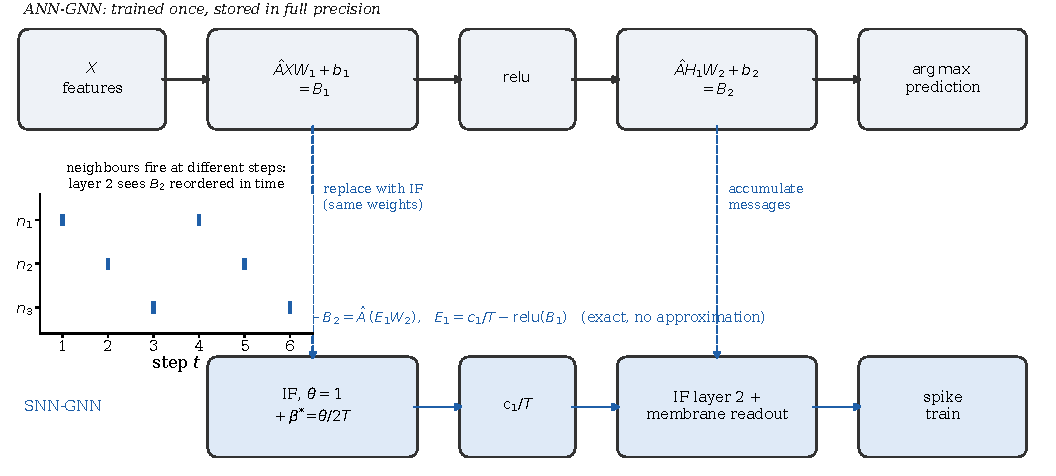
\includegraphics[width=\textwidth]{figures/fig1_framework.pdf}
\caption{The conversion and the feature that has no convolutional analogue. Top lane: train a
two-layer GCN once, then replace the rectifiers with IF populations and decode the accumulated
layer-2 membrane potential; a single trained model serves every latency $T$. Bottom lane: what
layer~2 actually integrates. In a convolutional network the operands of a layer are a fixed tensor,
so every channel of a receptive field advances on the same clock. In a graph the operand is the set
of neighbours $\{m\}$ of a node; each neighbour emits its rate on its own phase, so the partial sums
$\mathrm{inst}_{t}$ are not partial sums of $\Btwo$ in any order. The inset makes the point for one
node with three neighbours and $T=4$: the same total spike count, delivered in different orders,
gives different decisions, which is why the conversion error is a property of the neighbourhood and
not only of the layer.}
\label{fig:framework}
\end{figure*}

Substituting the definition of the layer-1 rate, $\cntone \coloneqq \sum_{t} s_{1,t}$, gives the
exact identity
\begin{equation}
\boxed{\;\Btwohat - \Btwo = \Ahat\left(\Eone W_{2}\right),
\qquad \Eone \coloneqq \cntone/T - \mathrm{relu}(\Bone)\;}
\label{eq:identity}
\end{equation}
\eqnref{eq:identity} is not an approximation and contains no assumption: it is what the shipped
simulation computes. The first consequence is that the conversion error is \emph{linear} in the
layer-1 rate error, passed through the same operator as the signal---so the graph does not merely
attenuate the error, it re-mixes it across the neighbourhood. Second, the error is invisible if one
inspects only layer-1 rates: $\Eone$ can be small elementwise while $\Ahat(\Eone W_{2})$ is large for
a particular node, because the neighbourhood sums $\Eone$ with weights $a_{n}[m]$. Third, and this
is the practical content of ``misalignment'', the sum in \eqnref{eq:layer2} is over
\emph{time-ordered} contributions $s_{1,t}$ from neighbours that have no reason to be time-aligned:
node $m$ may deliver its whole rate in the first two steps and node $m'$ in the last two, so the
partial sums $\mathrm{inst}_{t}$ are not partial sums of $\Btwo$ in any useful order. Averaging over
$T$ is what repairs the order, and the repair is exact only in the limit---at finite $T$ the residual
is $\Eone$.

\subsection{The IF unit as an exact floor quantiser}
\label{sec:lemma1}

For a constant current $c$ with $0 \le c \le \theta$, the membrane after $t$ steps is
$u_{t} = tc - \theta\,\mathrm{count}_{t}$ with $u_{t} \in [0,\theta)$, hence
\begin{equation}
\mathrm{count}_{T} = \left\lfloor \frac{Tc}{\theta} \right\rfloor,
\qquad U \coloneqq Tc - \theta\,\mathrm{count}_{T} \in [0,\theta),
\label{eq:floor}
\end{equation}
so the rate is $c - U/T$ and $\Eone = -U/T$. The three regimes are exactly what
the implementation does:
\begin{itemize}\itemsep1pt
\item $c < 0$: never fires, rate $0$; since $\mathrm{relu}(c) = 0$ as well, \emph{ReLU is implemented
for free} and contributes no error.
\item $0 \le c \le \theta$: rate $\lfloor Tc \rfloor / T$, error $-U/T$ of magnitude $< 1/T$.
\item $c > \theta$: saturates at one spike per step, rate $1$, error $1-c$ --- \textbf{unbounded}.
\end{itemize}
The third row is the only way the error escapes the $1/T$ regime, which is why an absolute threshold
needs justification. We give it in \secref{sec:fidelity}: with $\theta = 1$ and no global rescaling,
the fraction of $\mathrm{relu}(\Bone)$ exceeding the threshold is $0.00$--$0.01\%$ on the citation
graphs under GCN and mean aggregation, and $0.61$--$0.67\%$ under sum aggregation. A global
rescaling would suppress even that, but it would also destroy the very quantity the theory is about,
because it assumes $\rhon = 1$.

\subsection{The bias has a closed form}
\label{sec:bias}

Because the IF unit is deterministic, $\Eone$ is a deterministic function of $\Bone$; the
probabilistic content enters only through the population distribution of the residuals $U$. Under the
standard phase-randomisation assumption---$U[m,h]$ approximately uniform on $[0,1)$ and independent
across $(m,h)$---\eqnref{eq:floor} gives
\begin{equation}
\mathbb{E}[\Eone] = \beta - \frac{1}{2T}
\qquad\Longrightarrow\qquad
\betastar = \frac{\theta}{2T},
\label{eq:betastar}
\end{equation}
the unique bias that zeroes the systematic error, while the fluctuation half-width $1/(2T)$ is
unchanged by the bias. Two consequences separate cleanly. The bias does \emph{not} make the
conversion more accurate by shrinking noise; it removes a \emph{bias}, so its effect is largest where
the bias is largest relative to the margin, i.e.\ at small $T$. And the bias is
\emph{degree-weighted}: propagating the mean error through \eqnref{eq:identity} gives a margin shift
of $\rhon/(2T)\sum_{h} DW_{c}[h]$ for a rival class $c$, so a graph with large row sums suffers
proportionally more---which is why the correction matters more here than in vision, where the
analogous operator is row-stochastic. We verify the assumption rather than assert it: measured
$\mathrm{var}(U)$ is $0.082$ against the uniform value $0.083$, and $\mathbb{E}[U]$ is $0.481$
against $0.5$ (\secref{sec:theory}).

\subsection{Decoding: membrane, not count}
\label{sec:readout}

The obvious decoder counts output spikes. It has two defects that compound. The count is an integer,
so the logits live on a grid of spacing $1/T$; and a logit larger than one is clipped to one, so the
\emph{ordering} of large logits is destroyed even when their rates are correct. Both are artefacts of
decoding, not of the spike train: from \eqnref{eq:layer2}, the membrane potential satisfies
\begin{equation}
\mathrm{mem} = \cntone\,\theta + u = \sum_{t} \mathrm{inst}_{t},
\qquad \frac{\mathrm{mem}}{T} = \Btwohat,
\label{eq:memreadout}
\end{equation}
exactly, for the \emph{same} spikes. We therefore read out $\arg\max(\mathrm{mem})$. The decoder is
free---it uses the sub-threshold remainder that the count discards---and it removes the clipping
ceiling entirely, because $\mathrm{mem}$ is not bounded by $\theta$. The price is one accumulator per
class, which any neuromorphic core already has.

The claim has two boundaries. The ceiling we remove is the one \emph{counting} imposes; a decoder
that reads a continuous quantity does not have it, and we do not claim that conversion work using
analogue readout suffers from it---we claim that the rate-decoded conversions in the lineage we
build on do, and we measure the size of the effect rather than argue for it
(\secref{sec:ablate}). And the readout is only free because layer~2 already integrates a current;
reading that accumulator instead of the spike counter it drives costs nothing on any core that
implements an integrate-and-fire output layer, but it does require the accumulator to be visible,
which some event-driven interfaces hide.

\subsection{Margin recovery guarantee}
\label{sec:thm}

Fix a node $n$, let $c^{\star}$ be the ANN's argmax and $c$ a rival, and put
$DW \coloneqq W_{2}[:,c^{\star}] - W_{2}[:,c]$. Expanding \eqnref{eq:identity} with
$\Eone = \mathbb{E}[\Eone] + \xi$,
\begin{align}
\text{margin error}
&= \underbrace{\rhon \sum_{h} \mu_{h} DW[h]}_{\text{systematic}}
+ \underbrace{\sum_{m,h} a_{n}[m]\, DW[h]\, \xi[m,h]}_{\text{fluctuation}}
\label{eq:split}
\end{align}
where $\mu_{h}$ is the per-hidden-unit mean error. The fluctuation is a sum of independent bounded
terms of half-width $w$, so Hoeffding \citep{hoeffding1963probability} gives, with probability at
least $1-\delta$,
\begin{equation}
\left|\text{fluctuation}\right| \le w\,\anorm\,\lVert DW\rVert_{2}\sqrt{2\ln(2/\delta)} .
\label{eq:hoeffding}
\end{equation}
The factor is $\anorm$ ($0.469$ on Cora), not $\rhon$ (up to $5.75$): \eqnref{eq:hoeffding} is the
quantitative statement of ``the neighbourhood averages the quantisation error instead of accumulating
it''. Peeling out the saturated units of \secref{sec:lemma1} as an exactly computable term
$\sigma_{n}$ yields the guarantee.

\begin{theorem}[Margin recovery]
\label{thm:margin}
If, for every rival $c$,
\begin{equation}
\begin{split}
\Deltan \coloneqq {}&\Btwo[n,c^{\star}] - \max_{c \neq c^{\star}} \Btwo[n,c]\\
>{}& \left|\text{systematic}_{n}\right| + \sigma_{n}
+ w\,\anorm\,\lVert DW_{c}\rVert_{2}\sqrt{2\ln(2/\delta)},
\end{split}
\end{equation}
then $\arg\max \Btwohat[n,:] = \arg\max \Btwo[n,:]$ with probability at least $1-\delta$.
\end{theorem}

Equivalently $T = O(\anorm \lVert DW\rVert_{2} / \Deltan)$: the required latency is set by the
geometry of the neighbourhood and the class-weight separation, not by the graph size. $\betastar$
additionally removes the $\rhon\left|\sum_{h} DW_{h}\right|/(2T)$ term, which roughly halves the
required $T$ when the systematic part dominates---consistent with the observation that the bias helps
most at small $T$.

\subsection{Depth, and from the recursion to a prediction}
\label{sec:predict}

The identity of \eqnref{eq:identity} is stated for one hidden layer. It extends to $L$ without
approximation: summing the per-step input of hidden layer $l$ over $T$ steps and dividing by $T$
gives, for every $l$,
\begin{equation}
\hat{B}_{l}-B_{l}=(1-\alpha)\,\Ahat\,(E_{l-1}M_{l}),\qquad
E_{l}=\tfrac{1}{T}\mathrm{count}_{l}-\mathrm{relu}(B_{l}),
\label{eq:recursion}
\end{equation}
with $E_{0}=0$ because layer~1 is driven by the constant input, and $\alpha$ the weight of an initial
residual if the backbone has one. Taking norms, and using $\lVert\Ahat\rVert_{2}\le1$ together with
$\lVert D_{l}\rVert_{2}\le1$ for the ReLU active-set mask, the output error is bounded by
\begin{equation}
\lVert E_{L}\rVert\;\lesssim\;\sum_{j}\lVert\varepsilon_{j}\rVert\prod_{k>j}(1-\alpha)\lVert M_{k}\rVert_{2},
\qquad G\coloneqq\prod_{l}\lVert M_{l}\rVert_{2}.
\label{eq:amp}
\end{equation}
So depth enters the conversion error only through a product of per-layer spectral gains, and $G$ is
computable from the trained weights in milliseconds.

\paragraph{The layer-1 error is a quantisation error, not a modelling error.}
Each unit of the first layer emits $\lfloor T(c+\beta)/\theta\rfloor$ spikes in $T$ steps, so its rate
differs from its pre-activation by at most $1/(2T)$ plus whatever the bias fails to remove. The errors
of different units are driven by different weights and different threshold crossings, so they are
approximately independent, and a row of $E_{1}$ is a sum of $H$ independent terms. The active
hidden width $H$ is what the title calls the \emph{activation mass}: the number of active units
carrying quantisation error. Hence
\begin{equation}
\lVert E_{1}\rVert \;\approx\; \kappa\,\sqrt{H}\,/\,T ,
\label{eq:sqrtH}
\end{equation}
with $\kappa$ a constant of order one. \eqnref{eq:sqrtH} is a statement about a \emph{norm}, and it is
why widening an ANN is not free for its conversion: the error grows as the square root of the width
while the logit margin grows more slowly.

\paragraph{Propagation is a product of spectral gains.}
\eqnref{eq:amp} multiplies the layer-1 error by $G$ on the way to the logits. Combining the two, the
perturbation at node $n$ is a zero-mean random variable with scale
\begin{equation}
\sigma_{n} \;=\; \frac{c\,G}{T}\,\sqrt{H}\,\lVert a_{n}\rVert_{2}\,r_{L},
\qquad r_{L}=\Big(\tfrac{1}{C}\sum_{c}\lVert M_{L}[:,c]\rVert_{2}^{2}\Big)^{1/2},
\label{eq:sigma}
\end{equation}
where $a_{n}$ is row $n$ of $\Ahat$ and $r_{L}$ converts a hidden-space error into a logit-space one.
Everything in \eqnref{eq:sigma} except the single scalar $c$ is computed from the trained weights and
the graph.

\paragraph{A prediction, and one free parameter.}
A node keeps its label when the perturbation is smaller than half its margin, so
\begin{equation}
\widehat{\mathrm{acc}}(T) \;=\; \frac{1}{N}\sum_{n\,:\,\hat{y}_{n}=y_{n}}
\mathbb{P}\big(|\varepsilon_{n}|<\tfrac{1}{2}\Deltan\big),
\label{eq:predacc}
\end{equation}
with $\varepsilon_{n}$ centred at zero and scaled by \eqnref{eq:sigma}. The sum runs over the nodes the
ANN already classifies correctly: a node it gets wrong can only be rescued by noise, and counting that
would flatter the predictor. The consequence is a small systematic under-prediction, which we report
rather than correct.

We fit $c$ once, by grid search, on a set of training cells, and then predict cells the fit has never
seen. That is the difference between this section and \secref{sec:tight}: a bound is checked against
one run, whereas a prediction can be wrong about a run it did not see.

\paragraph{What the prediction is for.}
It converts three design questions into arithmetic on a trained model. (i) \emph{Will this backbone
convert?} Compute $G$; if $G\gg1$ the answer is no, and latency does not fix it, because
\eqnref{eq:sigma} falls only as $1/T$ while the error grows multiplicatively in depth. (ii) \emph{How
much latency?} Invert \eqnref{eq:predacc} for the smallest $T$ reaching a target. (iii) \emph{Should I
widen?} \eqnref{eq:sqrtH} says the error grows as $\sqrt{H}$ while the margin grows with the ANN's
confidence; which wins is measurable before the conversion is run.

\subsection{Complexity and deployment}
\label{sec:complexity}

Training is ordinary GCN training, once. Deployment at latency $T$ costs $T$ sparse neighbourhood
aggregations of binary vectors plus $T$ dense products $s_{1,t}W_{2}$; the spike budget is
$\sum\cntone + \sum \mathrm{count}_{2}$. Because the weights do not depend on $T$, a single trained
model serves every latency, and the accuracy--latency curves of \figref{fig:acc} are obtained by
re-running the same weights. This is the structural advantage over direct training, which must be
re-run---including its backward pass---for each $T$.
